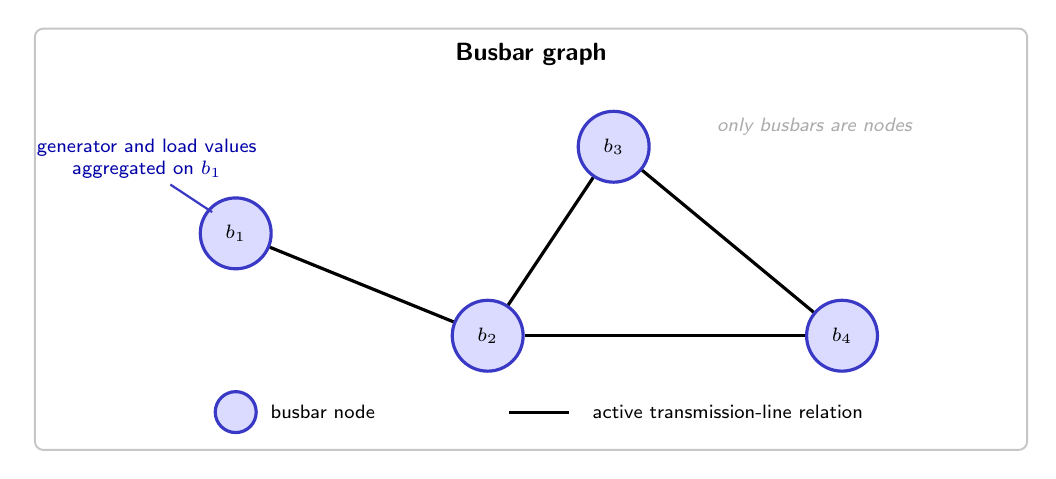
\begin{tikzpicture}[
  x=1cm,
  y=1cm,
  font=\sffamily,
  busbar/.style={
    circle,
    draw=blue!55!gray,
    fill=blue!14,
    line width=1.15pt,
    minimum size=9mm,
    inner sep=0pt,
    font=\scriptsize\sffamily
  },
  physical/.style={draw=black, line width=1.15pt},
  panel/.style={draw=gray!45, rounded corners=3pt, line width=0.7pt},
  title/.style={font=\small\bfseries\sffamily},
  note/.style={font=\scriptsize\sffamily, align=center},
  muted/.style={font=\scriptsize\itshape\sffamily, align=center, text=gray!65}
]

\path[panel] (0,0) rectangle (12.6,5.35);
\node[title] at (6.3,5.02) {Busbar graph};

% The same four-busbar network is reused in the next two figures.
\node[busbar] (b1) at (2.55,2.75) {$b_1$};
\node[busbar] (b2) at (5.75,1.45) {$b_2$};
\node[busbar] (b3) at (7.35,3.85) {$b_3$};
\node[busbar] (b4) at (10.25,1.45) {$b_4$};

\draw[physical] (b1) -- (b2);
\draw[physical] (b2) -- (b3);
\draw[physical] (b3) -- (b4);
\draw[physical] (b2) -- (b4);

\node[note, text=blue!65!black] at (1.42,3.70)
  {generator and load values\\aggregated on $b_1$};
\draw[draw=blue!55!gray, line width=0.8pt] (1.72,3.37) -- (2.25,3.02);

\node[muted] at (9.90,4.10)
  {only busbars are nodes};

% Compact legend.
\node[busbar, minimum size=5.2mm] at (2.55,0.48) {};
\node[note, anchor=west] at (2.87,0.48) {busbar node};
\draw[physical] (6.02,0.48) -- (6.78,0.48);
\node[note, anchor=west] at (6.96,0.48)
  {active transmission-line relation};

\end{tikzpicture}
